\section{Thiết lập thí nghiệm}
Phần này mô tả chi tiết các thiết lập và quy trình triển khai và đánh giá cho bài toán đa robot phối hợp đẩy vật. Thí nghiệm được thực hiện dưới dạng mô phỏng trong không gian 2D, sử dụng ngôn ngữ lập trình Python. Ba vật thể đa giác với ba hình dạng khác nhau, bao gồm đa giác lồi và không lồi được sử dụng để đánh giá khả năng của các phương pháp dưới các tình huống khác nhau. 

\subsection{Cấu hình robot}
Đồ án thực hiện thí nghiệm 4 robot, số lượng này có thể tăng hoặc giảm trong quá trình để thể hiện tính chất linh hoạt và mở rộng của thuật toán. Tham số của robot được chọn như sau: kích thước robot được chọn $r_r$ = 15 cm, lực pháp tuyến tối đa mỗi robot có thể tác dụng lên vật là $f_\text{max}$ = 50N trong pha đẩy vật , pha khám phá giả định $f_\text{max}$ = 150N. Khoảng cách an toàn đỉnh $d_s$ và khoảng cách an toàn tối thiểu giữa các robot $d_\text{min}$ lần lượt được thiết lập là 0.1m và 0.2m. Trong minh họa, do hình dạng của robot vốn không ảnh hưởng đến giải thuật, ràng buộc khoảng cách được đảm bảo bằng hệ số $d_\text{min} > r_r$ nên thay vì được biểu diễn bằng hình tròn, robot sẽ được minh họa bằng các tam giác cân có đường cao vuông góc với cạnh tiếp xúc để thể hiện hướng đẩy. 

\subsection{Môi trường thí nghiệm}
Môi trường thì nghiệm là một vùng không gian trống kích thước 12x12m, trong đó có một vật thể cần thao tác. Vật thể được biểu diễn bởi một mảng các vector hai chiều với đơn vị là m, trong đó mỗi vector $(x_i,y_i)$ thể hiện vị trí tương đối của một đỉnh $i$ so với khối tâm.



Ba vật thể được chọn lần lượt có hình chữ nhật, hình chữ T và hình ngôi sao (Hình \ref{fig:shapes})với khối lượng được lấy chung là 15kg, trong đó hai vật đầu tiên có khối tâm được lấy khác với tâm hình học.
\begin{figure}[h]
    \centering
    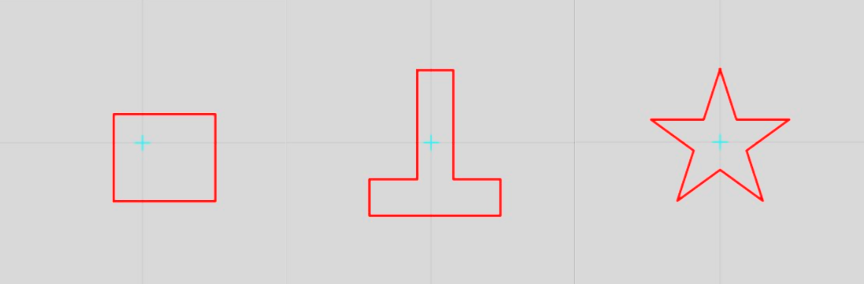
\includegraphics[width=1\textwidth]{chapter2/image/shapes.png}
    \caption{Ba vật thể được dùng trong thí nghiệm} 
    \label{fig:shapes}
\end{figure}

Thí nghiệm sẽ tập trung mô tả khả năng tạo cấu hình và sinh ra lực đẩy theo một số các wrench đơn lẻ được thiết lập sẵn và khảo sát tính khả thi. Ngoài ra, đồ án sẽ thử đẩy vật theo một quỹ đạo được thiết kế để thể hiện rõ các đặc trưng của chuyển động tịnh tiến và chuyển động xoay đơn lẻ, cũng như sự kết hợp của cả hai. Cụ thể, đầu tiên vật di chuyển từ vị trí $(0,0,0)$ đến vị trí $(2,0,0)$, sau đó tiến hành xoay tại chỗ một góc 90 độ đến vị trí $(2,0,90)$. Tiếp đó, vât vừa di chuyển theo đường thẳng vừa xoay đến vị trí $(2,2,0)$, cuối cùng di chuyển theo đường chéo về lại vị trí ban đầu.